\documentclass[../index.tex]{subfiles}

\begin{document}

\chapter{REQUIREMENT ANALYSIS AND DESIGN}

This chapter will examine the proposed project requirements and system design. Identifying project
requirements and defining the proposed system design are mandatory to successfully deliver the
project objectives and functionalities.

\section{Requirement Analysis}

Unified Modeling Language (UML) is chosen as a method to analyze the project requirements. UML is a
graphically based notation, which is developed by the Object Management Group as a standard means of
describing software-oriented designs. It contains several different types of diagrams, which allow
different aspects and properties of a system design to be implemented.

% However, for this particular project, only a few of UML diagrams will be used. This due to the
% project development does not involve any creation of new software or interface. Rather, this
% project implements off-shelf software solutions in a defined hardware.

The functional requirements are described using UML use case diagram and activity diagram. The
non-functional requirement will review the performance, usability, availability, reliability, and
security aspect of the system.

\subsection{Functional Requirement}

This section will outline the specific features, capabilities, and behavior that the software system
should possess in order to fulfill its intended purpose and meet the needs of its users. The
functional requirements describe what the system should do, rather than how it should be
implemented.

\subsubsection{Use Case Diagram}

Use case diagram is a visual depiction of a user's possible interactions with a certain system. A
use case diagram defines varying use cases and different types of users the system has and commonly
delivered with other types of diagrams as well. Use case diagram offers thorough summary of the
entire system with simple illustration. Use case diagram is also considered as the perfect method to
provide the overall view of the system at the early stage \cite{Shen2003FormalizationTA}.

\begin{figure}[h]
  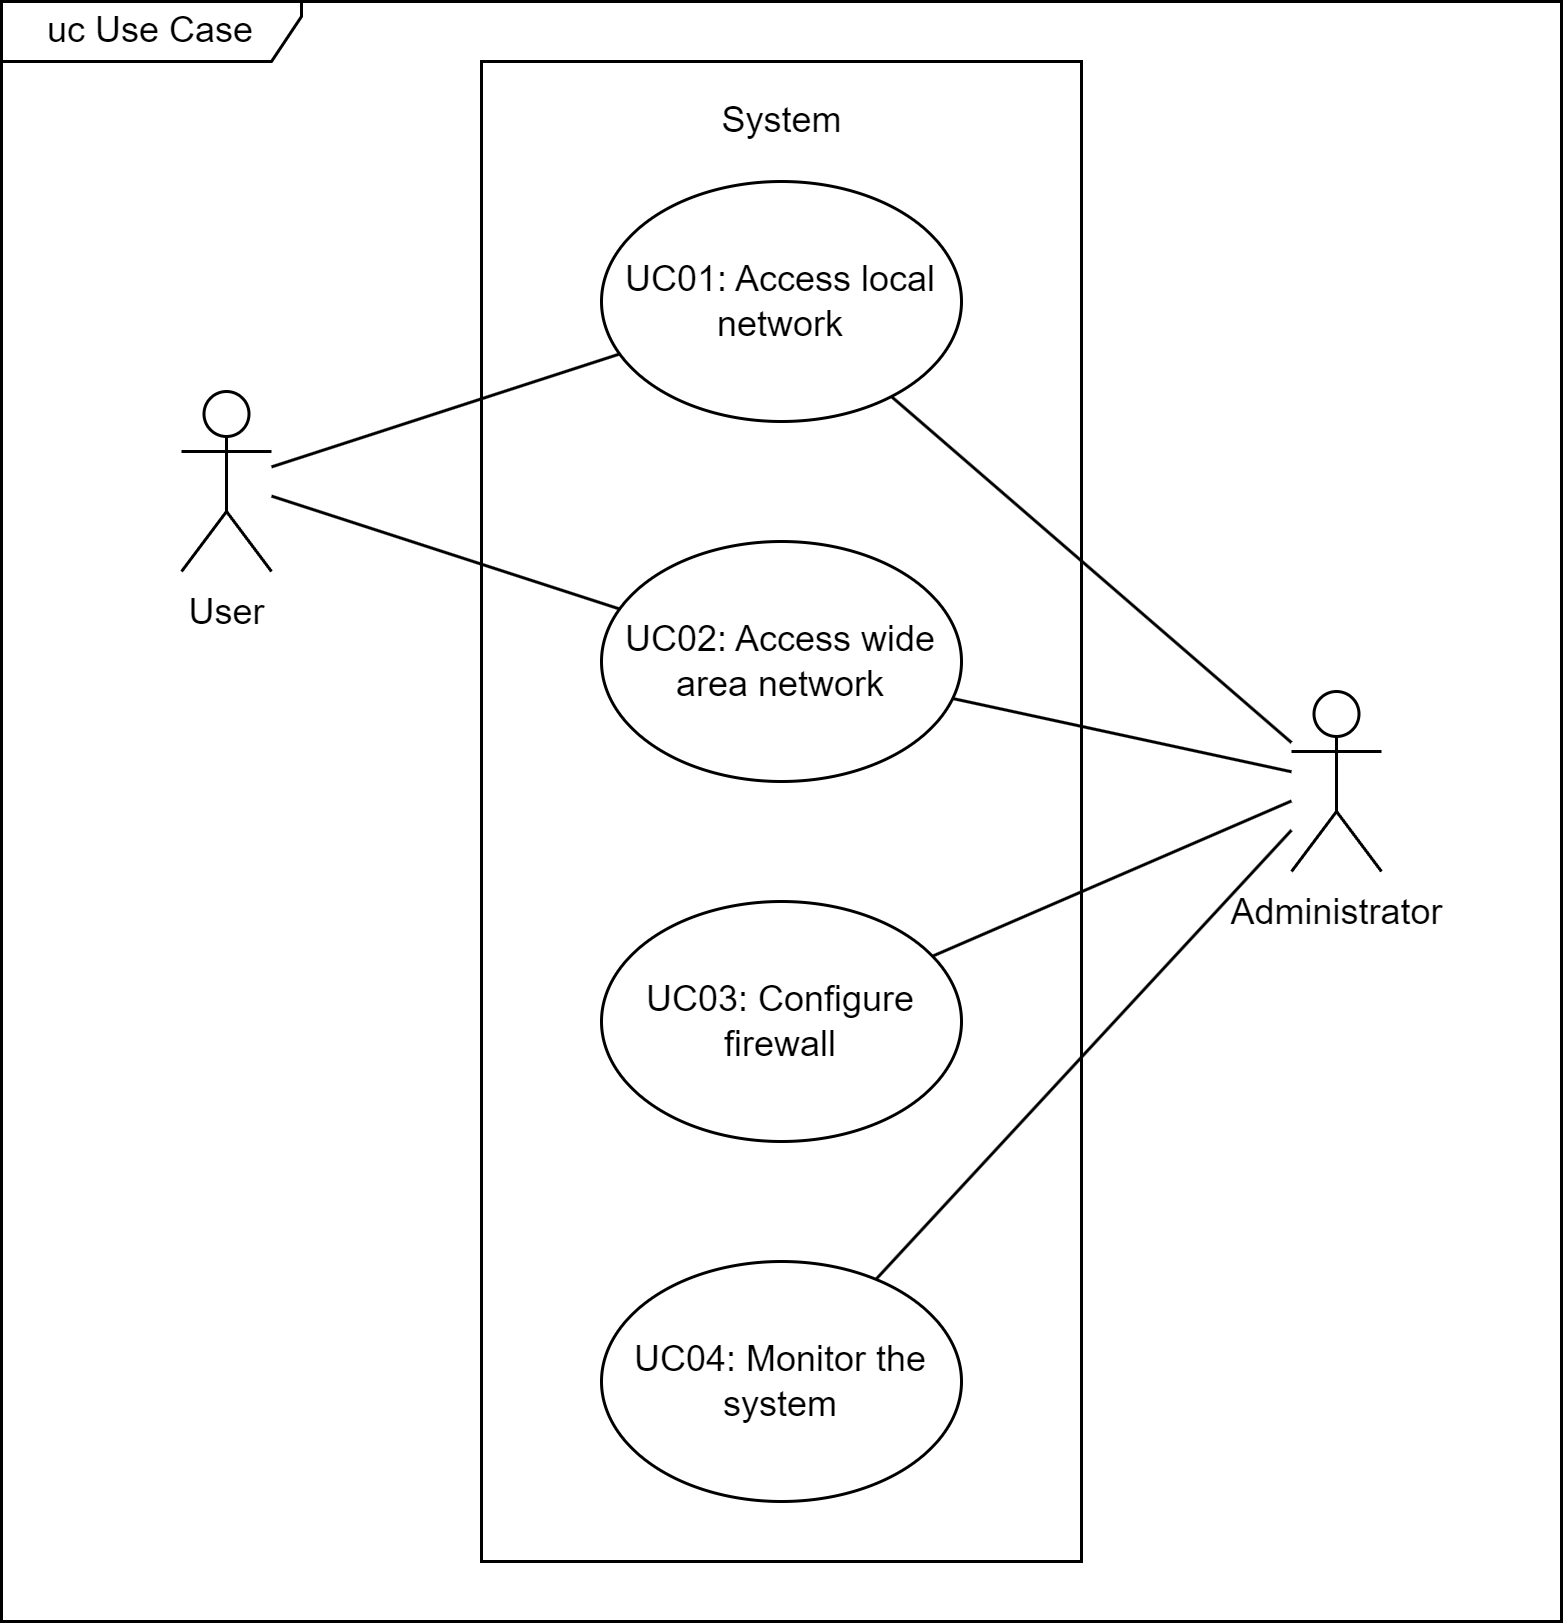
\includegraphics[width=\textwidth]{../assets/use_case.drawio_2.png}
  \caption{Use case diagram of the proposed system}
  \label{fig:use_case}
\end{figure}

\Cref{fig:use_case} shows the use case diagram of the proposed system. The use case diagram is
designed based on the result of the requirement analysis phase. In the proposed system, there exist
three actors which are the user, the system, and the administrator. Four use cases were also
defined, which are accessing local network, accessing wide area network, configuring the firewall,
and monitoring the system. In addition, it followed by a table which list the brief use case
description.

\begin{table}[H]
  \begin{tblr}{hlines,width=\textwidth,colspec={|X[l,m]|X[l,m]|}}
    \SetCell[c=1]{c} Use Case & \SetCell[c=1]{c} Description \\
    UC01: Access local network & User access another device which exists in the local network \\
    UC02: Access wide area network / Internet & User access the Internet \\
    UC03: Configure System & Administrator configure the system using the proposed Ansible code \\
    UC04: Monitor system & Administrator monitor the system metrics and logs \\
  \end{tblr}
  \caption{Brief description of use case diagram}
  \label{table:use_case}
\end{table}

\Cref{table:use_case} lists all of the use cases identified for the proposed system. The use case
description provides the flow of each use case, alternative flow, the precondition that should be
fulfilled as well as post conditions based on the outcome of the flow. The purpose of defining the
use case description is to present the overall view of the system function and reaction to the user
and administrator. In the proposed system, there are 4 use cases in total which detailed more in
Appendix A.

\begin{table}[H]
  \begin{tblr}{hlines,measure=vbox,width=\textwidth,colspec={|l|X[l,m]|}}
    Use case & Access local network \\
    ID & UC01 \\
    Description & User access another device which exists in the local network \\
    Actor & User, System \\
    Related use case & - \\
    Precondition & User's device is connected to the local network \\
    Normal flow &
    \begin{enumerate}
      \item The use case starts whenever user is trying to communicate or access a device in the
        local network

      \item The system receives the request packet from user's device

      \item The system forwards the packet to the appropriate destination, in this case it is the
        device which the user wants to access

      \item The destination device receives the packet

      \item The destination device sends the response packet to the system

      \item The system forwards the packet to appropriate destination, in this case it is the user's
    \end{enumerate} \\
    Alternative flow & - \\
    Post condition &
    \begin{enumerate}
      \item Success condition
        \begin{enumerate}
          \item The user receives the response from the device
        \end{enumerate}
        \item Failure condition
          \begin{enumerate}
            \item The user fails to receive the response from the device

            \item The system drops the packet
          \end{enumerate}
    \end{enumerate} \\
  \end{tblr}
  \caption{Use case description of Access Local Network}
  \label{table:use_case_1}
\end{table}

\subsubsection{Activity Diagram}

As stated by \cite{10.1109/APSEC.2004.55}, activity diagram could be used to model the dynamic
aspects of a group of objects, making it a perfect method to describe the fulfillment of the
operation in the design phase. Activity diagram also suitable to describe the sequence of the
activities among the existing objects in the control flow during the implementation of an operation.
In addition, activity diagram could be used to describe the relationship between the activity and
the object in the system flow as well as the change of state of object in the object flow as the
activity being executed. The following figure shows the activity flow of access local network. The
complete activity diagram of the system is enclosed in Appendix A.

\begin{figure}[h]
  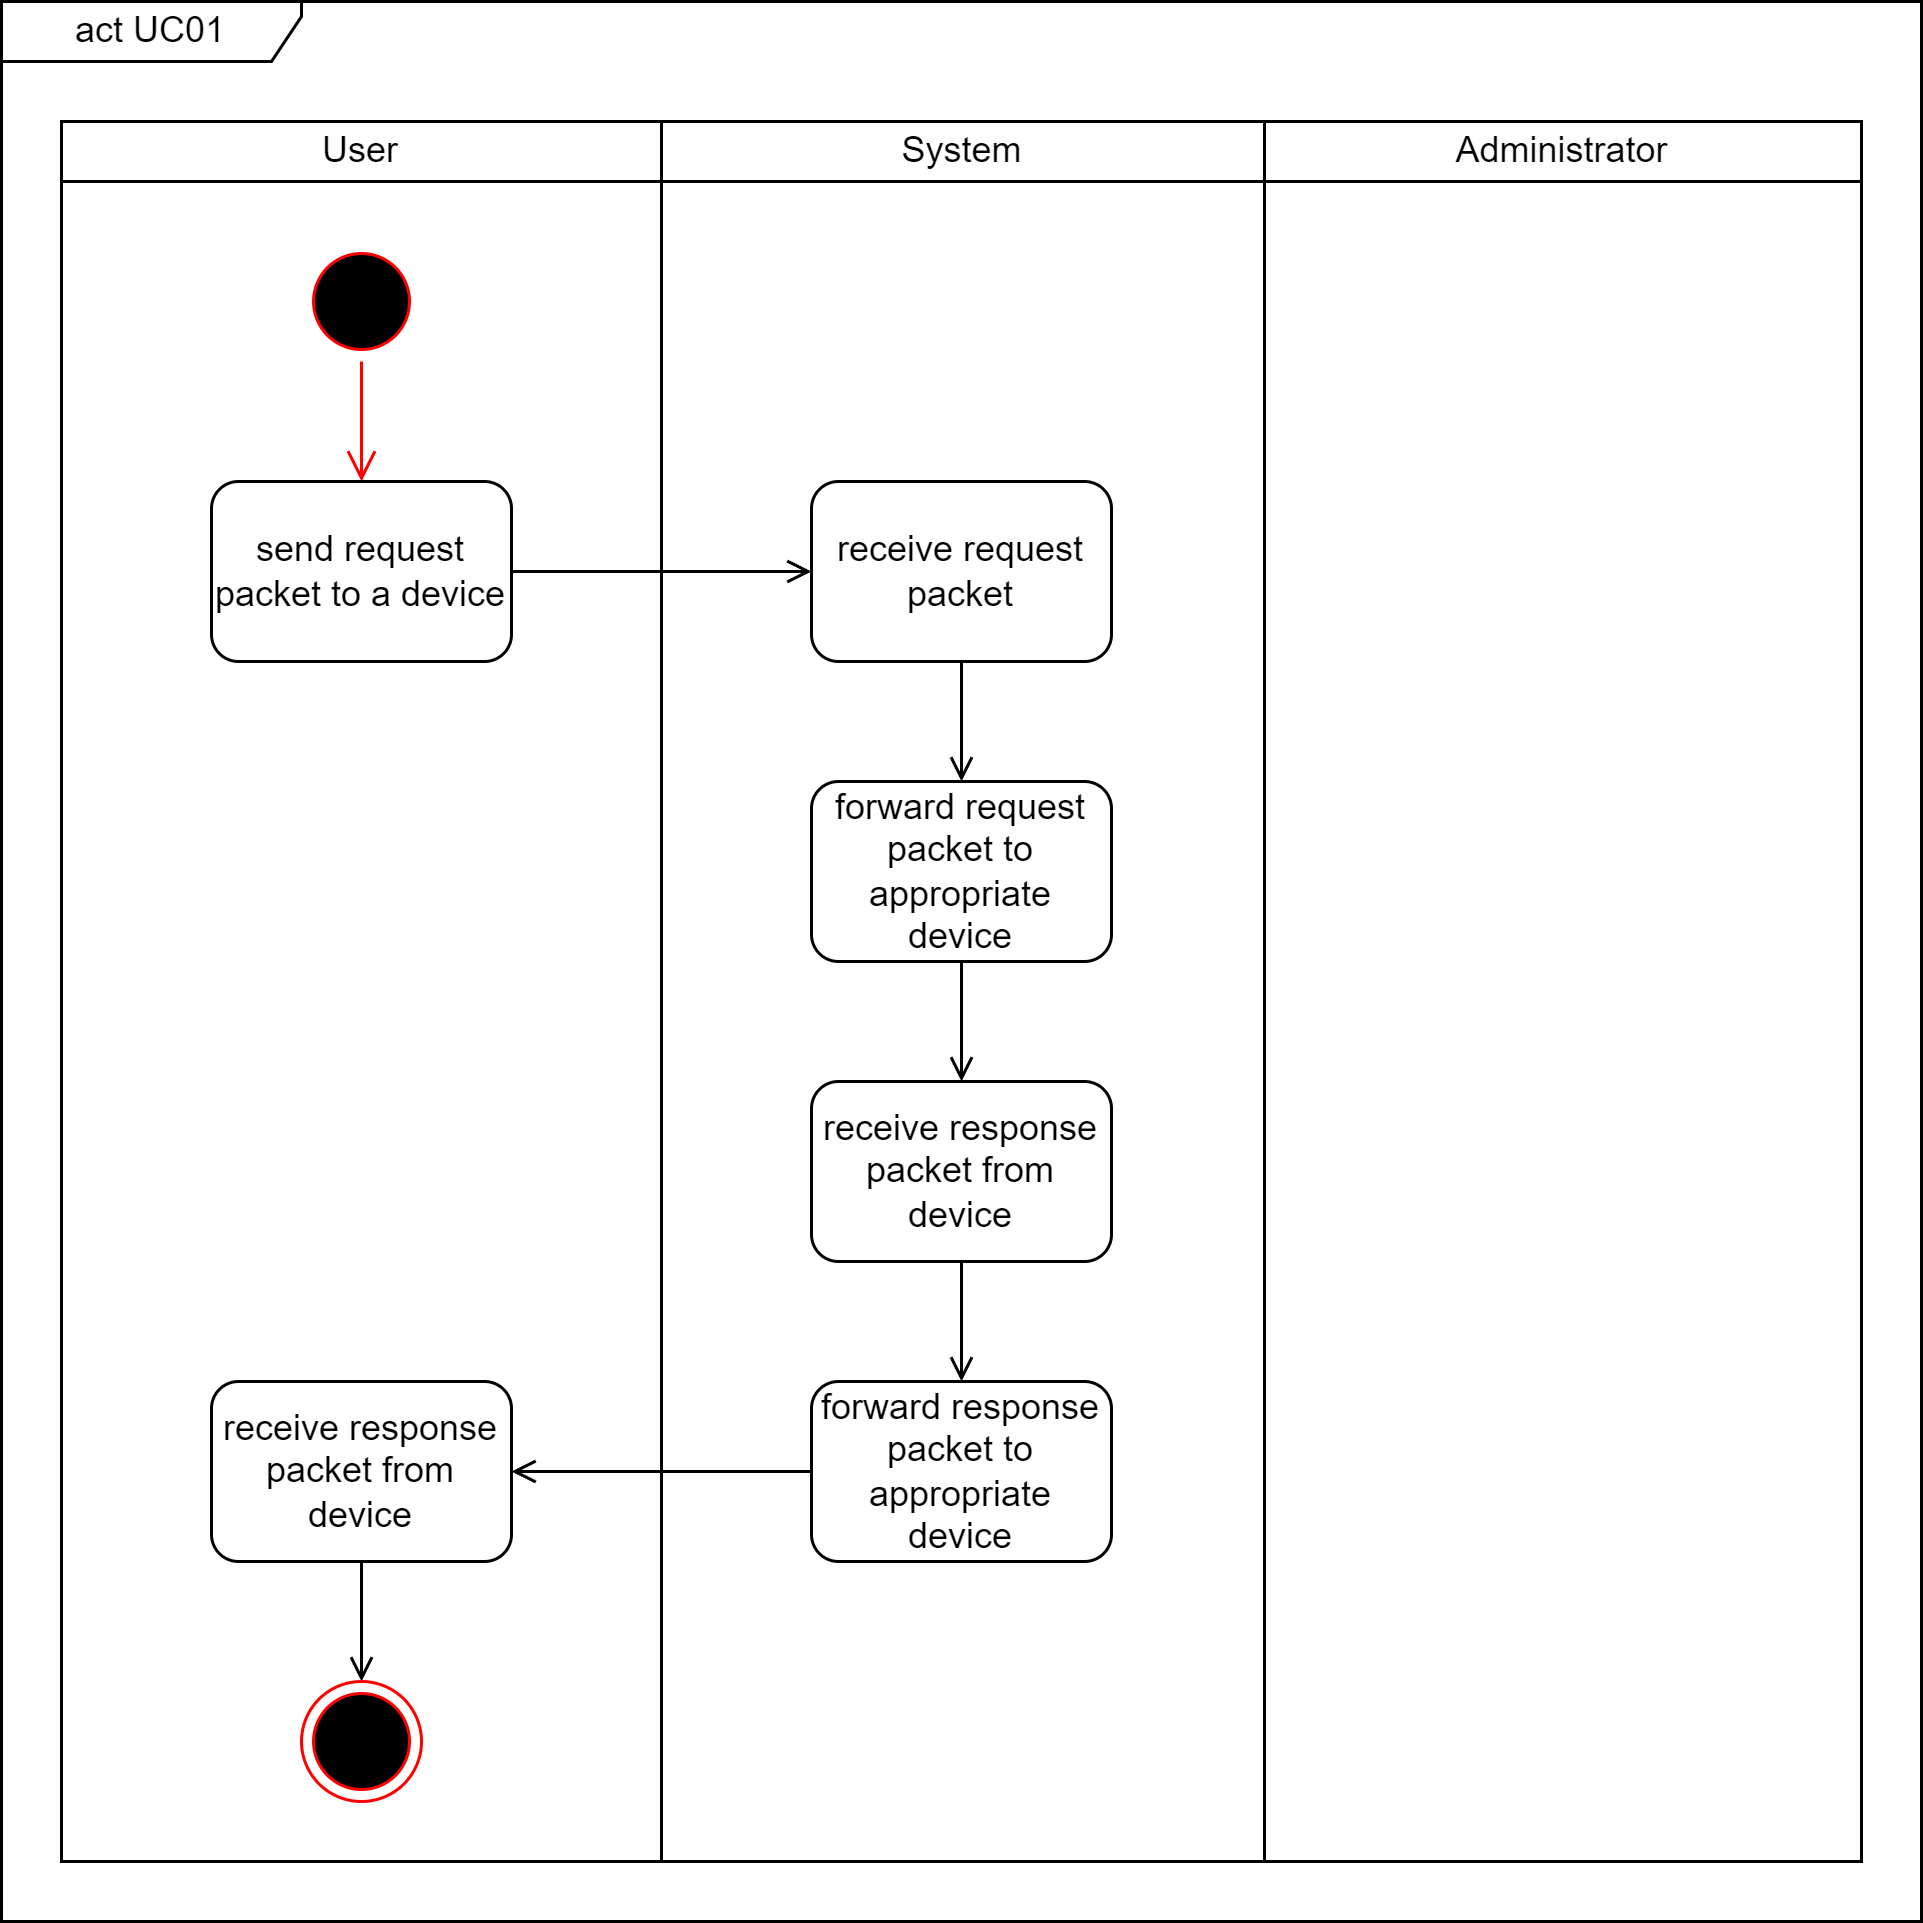
\includegraphics[width=\textwidth]{../assets/activity_diagram.drawio.png}
  \caption{Activity diagram of Access Local Network}
  \label{fig:activity_diagram_1}
\end{figure}

\subsection{Non-functional Requirement}

The non-functional requirement describes the measurement of quality of the system, consisting of
system performance, usability, availability, reliability, and security

For the system performance, the developed system should be able to transmit over 900 Mbps. This is
due to the NIC used, which is limited to 1 Gbps. As for the system usability, the administrator
should be able to modify the configuration of the firewall based on their requirement. As the system
will act as both internet router and network firewall without high availability (HA), the system is
expected to be able to run 24 hours a day, seven days a week. The error budget is only allocated for
the system maintenance. Aside securing the local network, the system also required to have certain
kind of self-security functionality to be able to defend itself from attacks

% \section{Project Design}
\section{Infrastructure Design}

The system will utilize Proxmox VE which act as server management platform as its base. Proxmox VE
provides KVM hypervisor, storage and network virtualization for the system. The Proxmox VE will
manage virtualised OPNsense host and local Kubernetes cluster in parallel. The OPNsense host will
provide the main network firewall and routing capabilities. The Pi-hole will be deployed on an LXC
container.

\begin{figure}[h]
  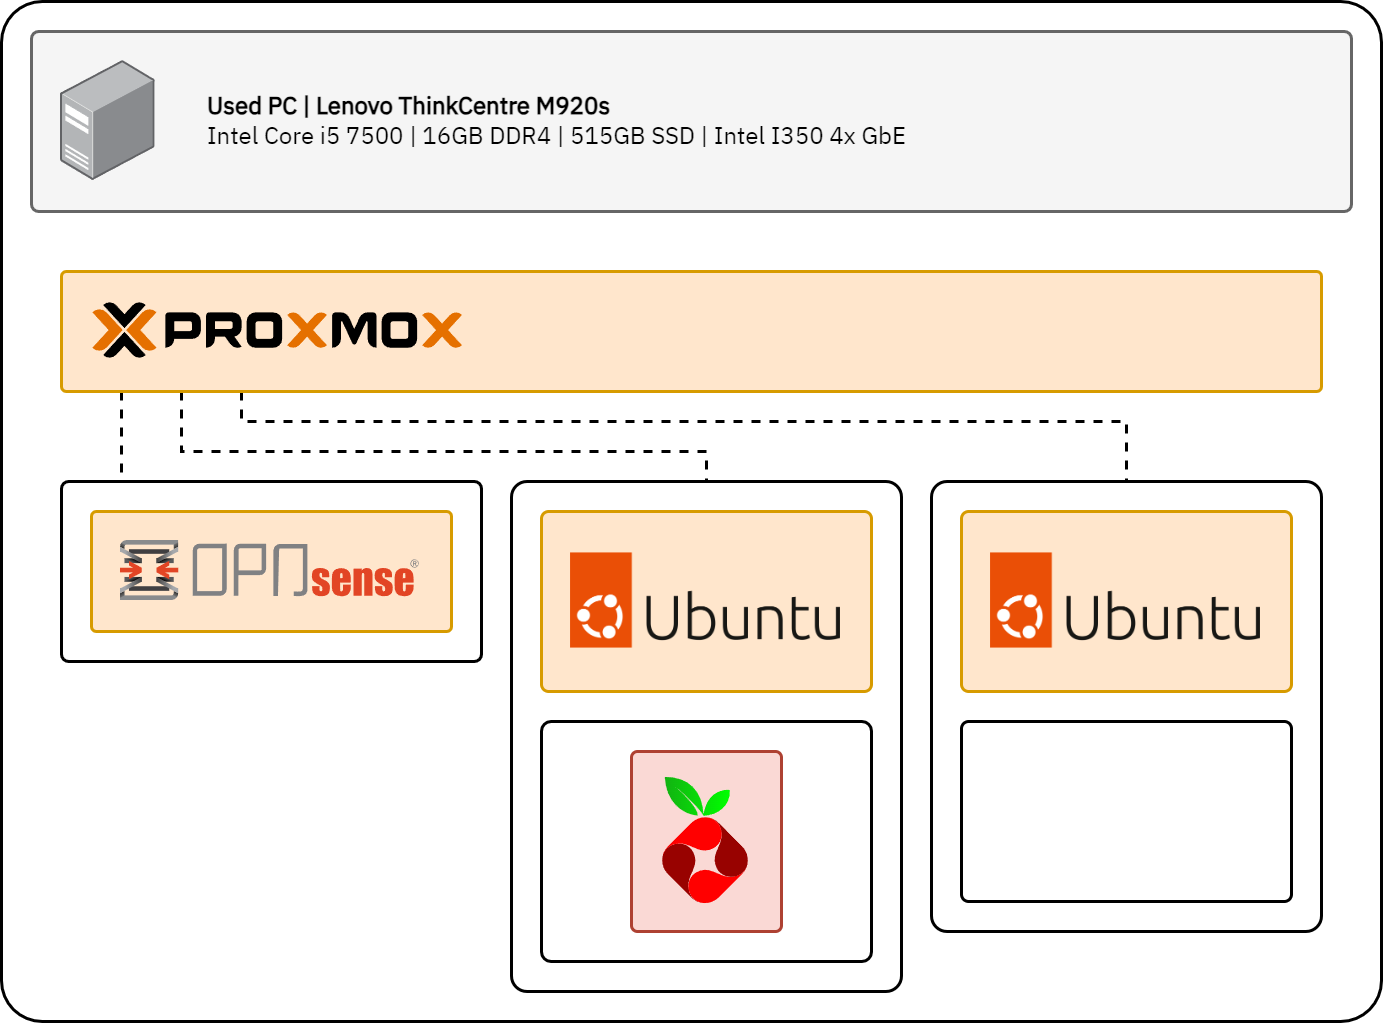
\includegraphics[width=\textwidth]{../assets/project_design.drawio.png}
  \caption{Proposed system infrastructure design}
  \label{fig:project_design}
\end{figure}

\section{Summary}

This project uses different approach for its requirement analysis and system design. This chapter
does not include proposed software design as the proposed system development does not involve the
creation of a new software or application, rather designing and re-purposing or configuring a
hardware to make it usable as alternative for firewall appliances which have significantly higher
price tag.

\end{document}
